\documentclass[sigconf]{acmart}

\usepackage{algorithmic}
\usepackage{algorithm}
\usepackage{hyperref}

\begin{document}

\title{Lab 5 Exercise -  A little Linear Regression}
\author{Luke McClure}
\email{29573904}

\maketitle
\pagestyle{myheadings}

\section{An initial attempt}
As this is a regression problem MSE was used as the loss function for all models.
\subsection{A simple CNN baseline}
When considering the connections between the convolutional and fully connected layers, and therefore the learnable parameters within the fully connected layers (9830786 to be exact), it is no surprise that the model starts to overfit to the data relatively quickly as seen in \autoref{fig:CNN1}.

\begin{figure}[h]
    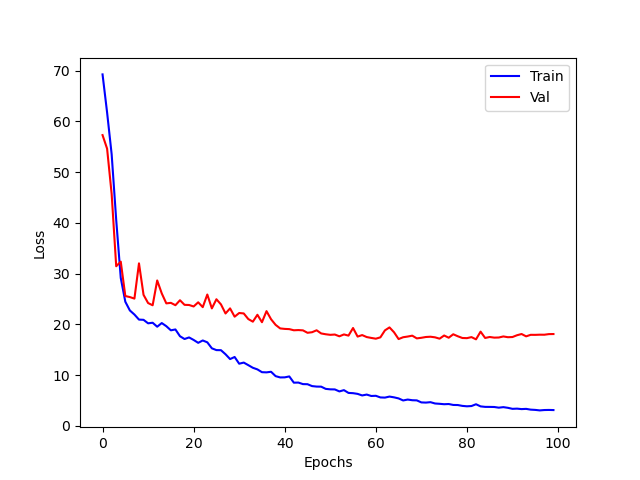
\includegraphics[scale=0.35]{../CNN1.png}
    \caption{CNN Baseline}
    \label{fig:CNN1}
\end{figure}

The validation and training losses start to diverge at around 25, with the final validation loss at close to 20 while final training loss is closer to 5.

\section{An second attempt}
\subsection{A simple CNN with global pooling}

By using a global max pooling layer between the convolutional and fully connected layers we can cut down on the number of learnable parameters, while also abstracting out detail from the image.
This vastly reduces the problem of the model overfitting to data, as is shown in \autoref{fig:CNN2}.
\begin{figure}[h]
    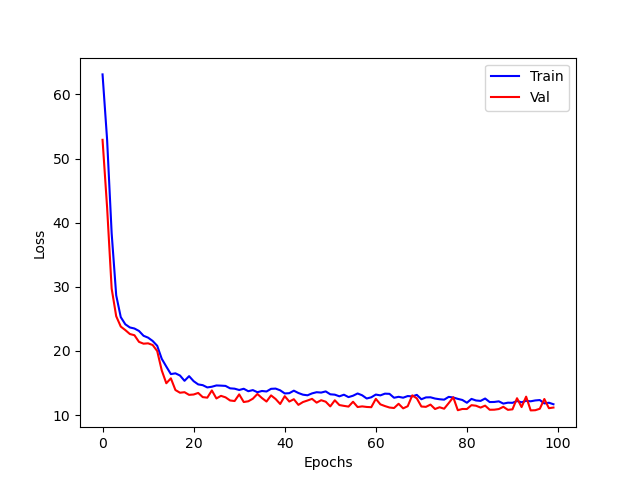
\includegraphics[scale=0.35]{../CNN2.png}
    \caption{CNN with global pooling}
    \label{fig:CNN2}
\end{figure}
Both training and validation losses drop to around 12 with the global max pooling, with the two staying fairly coupled even through bumps of the validation loss.
\section{Something that actually works?}
\subsection{Let's regress}

This model performs much better than previous, avoiding the overfitting issues and with losses dropping to close to 5 as seen in \autoref{fig:CNN3}.
\begin{figure}[h]
    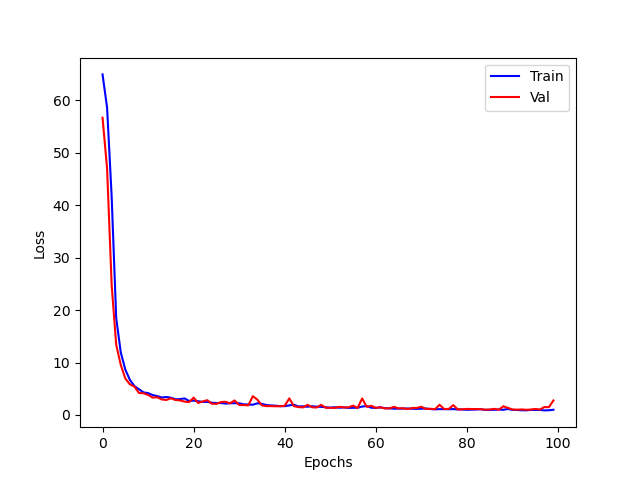
\includegraphics[scale=0.37]{../CNN3.png}
    \caption{CoordConv}
    \label{fig:CNN3}
\end{figure}

The third CNN is an architecture known as CoordConv, the other input channels are designed to let the network know where it is in Cartesian space.
By providing a grid of the x coordinates in one input channel and a grid of the y coordinates in the other hardcoded input channel the filter is able to pinpoint exactly where the points of the line are.
\begin{figure}[h]
    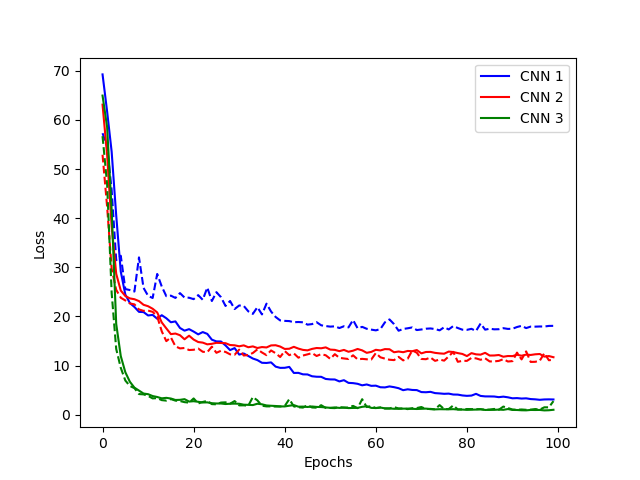
\includegraphics[scale=0.35]{../ALL.png}
    \caption{All CNN's compared (- train, -- validation)}
    \label{fig:ALL}
\end{figure}

\begin{center}
    \begin{tabular}{| c c |}
        \hline
        CNN & Test Loss \\ 
        \hline\hline
        CNN Baseline & 19.5 \\
        CNN with global pooling & 14.1\\
        CoordConv & 3.21\\
        \hline      
    \end{tabular}
\end{center}
\end{document}
\endinput